\chapter{Nearest Neighbor}
\label{cha:nearest_neighbor}

For Nearest Neighbor, we present the description of the algorithms and functions we have used to complete Nearest Neighbor.\\
We first tried to solve the reconstruction of the curve with only a Nearest Neighbor algorithm.\\
We start by giving some definitions, followed by a functional description of the algorithm, and finally a running time analysis. \\
TODO: REWRITE! We begin each section with a short introduction to the algorithm, followed by definitions and their proofs. Then a functional description of the algorithm is given. We conclude with a running time analysis of the algorithm.\\
After each algorithms we give functions which are used by the preceding algorithm.\\

  \section{Lexicographic Smallest}
  \label{sec:lexicographic_smallest}

    \subsection{Definitions}
    \label{sub:definitions}
      \begin{definition} \label{def:ls}
          Given a set $S$ with $n$ points, LexicographicSmallest returns the lexicographic smallest point in $S$.
      \end{definition}


    \subsection{Functional Description}
    \label{sub:functional_description}
      For the given set $S$ of $n$ points, the algorithm starts by selecting the first point in $S$ and compares its x-co\"ordinate with the x-co\"ordinate of the other points in $S$, until a smaller x-co\"ordinate is found. This point becomes the new lexicographic smallest and the algorithm continues comparing moving right of this point in the array.\\
      When in a comparison the two x-co\"ordinates of the two points are equal, the point with the smaller y-co\"ordinate becomes the lexicographic smallest.\\
      When all $n$ points are processed, the index of the lexicographic smallest point is returned.

    \subsubsection{Proof of correctness}
    \label{ssub:proof}
      \noindent The Lexicographic Smallest algorithm compares all the x-co\"ordinates of the points in $S$ and keeps track of the smallest until now. When there are two x-co\"ordinates with the same value, the point with the smaller y-co\"ordinate becomes the lexicographic smallest.\\ When all points are processed, the lexicographic smallest point of $S$ is found.
    

    \subsection{Running Time Analysis}
    \label{sub:running_time_analysis}
      As follows from the functional description, the algorithm processes each point exactly once.\\
      So the running time is $O(n)$.


  \section{Nearest Neighbor}
  \label{sec:nearest_neighbor}

    \subsection{Definitions}
    \label{sub:definitions}
      \begin{definition} \label{def:nn}
          Given a set $S$ of $n$ input points, NearestNeighbor returns the nearest neighbor of $n-1$ points in $S$.
      \end{definition}
      
    \subsection{Functional Description}
    \label{sub:functional_description}
    
      \begin{figure}
        \begin{tabular}{l r}
          \textbf{NearestNeighbor}$(P)$                                               & \\
          $ls \gets$ \textbf{LexicographicSmallest}$(P)$                              & \\
          $p \gets P[ls]$                                                             & \\
          \textbf{for} $i \gets 0$ \textbf{to} $|P| - 2$ \textbf{do}                  & \\
          \qquad $P \gets P \backslash \{ p \}$                                       & \\
          \qquad $d \gets \infty$                                                     & \\
          \qquad $q \gets p $                                                         & \\
          \qquad \textbf{for} $j \gets 0$ \textbf{to} $|P| - 1$ \textbf{do}           & \\
          \qquad \qquad \textbf{if} \textbf{distance}$(p, P[j]) < d$ \textbf{then}    & \\
          \qquad \qquad ~~ $d \gets$ \textbf{distance}$(p, P[j])$                     & \\
           \qquad \qquad ~~ $q \gets P[j]$                                            & \\
           \qquad \qquad \textbf{fi}                                                  & \\
           \qquad \textbf{od}                                                         & \\
           $S \gets S \cup \{ p \}$                                                   & \\
           $p \gets q$                                                                & \\
           \textbf{od}                                                                & \\ \hline \hline
           \qquad \qquad \qquad\qquad\qquad\qquad\qquad \textbf{Total }  & $O(n^{2})$
         \end{tabular}
         \label{fig:NearestNeigborcode}
         \caption{The pseudo code of NearestNeighbor}
      \end{figure}
    
      The Nearest Neighbor Algorithm works as follows:\\
      We have a array $A$ of $1$ to $n$ points and one empty array $B$ which has the same length.\\
      We choose the lexicographic smallest point (see \ref{ref:ls}), say $p$ and remove this point $p$ from $A$ and place it in $B$.\\
      This point will be our starting point. Next we measure the lengths between this point
      and all the remaining points in $A$ and we choose the point with the smallest distance to this point.
      This closest point we will call point $q$.\\
      Now that we have found the nearest neighbor of our starting point, we move $q$ from $A$ to $B$. We repeat this finding the smallest process on $q$, meaning for $q$ we look through all remaining points in $A$ for $q$'s nearest neighbor. This new point will be removed from $A$ and added to $B$. Now $r$ becomes the nearest neighbor of $q$ and we repeat this process until all points except for the last in $A$ have been processed (the last point has no nearest neighbour of it's own, being the last point in the set).

    \subsubsection{Proof of correctness}
    \label{ssub:proof}
      the Nearest Neighbor algorithm begins with removing $p$ from $S$ and calculates the distances between this point $p$ and the other points in $S$ and keeps track of the smallest point processed until now.\\ The point $q$ with the smallest distance to $p$ becomes the nearest neighbor of $p$ and is removed from $S$.
      Then the algorithm computes the nearest neighbor of $q$, say $r$, in the same way as for $p$.\\
      This goes on until the nearest neighbor of the $n-1^{th}$ point is processed; the nearest neighbor of this point is the only point left in set $S$: the $n^{th}$ point.\\
      So Nearest-Neighbor returns the nearest neighbor for each of the $n-1$ points in a set of $n$ points.

    \subsection{Running Time Analysis}
    \label{sub:running_time_analysis}
      Proving the running time for NearestNeighbor is pretty straight forward. There are only three lines that are not constant time; lines 1, 3 and 7. \\
       Line 1 uses a function that searches for the lexicographic smallest for its given input set. As proven in section \ref{ref:ls} this takes $O(n)$ time.\\
       Line 7 starts a for loop that looks through all remaining elements in the set $P$ looking for the smallest distance between point $j$ and given point $p$. This comparison is done in constant time and does not affect the running time of the for loop. In the first run, this for loop needs to go through the most number of elements, namely $n-1$ elements. The running time of this loop is $O(n)$. \\
       Line 3 starts the for loop that runs through all elements in the set, minus the last element. Thus, this takes $O(n-1)$. We need to take into account the nested for loop and finding the lexicographic smallest point, this makes the total running time: \\
       $O(n-1) * O(n) + O(n) =  O(n^{2} - n ) + O(n) = O(n^{2})$ \\
       Thus \textbf{NearestNeighbor} runs in $O(n^{2})$.

  \section{Experimental evaluation}
  \label{sec:experimental_evaluation}
    \subsection{Running time}
    We first tested our algorithm on randomly generated points (solely for determining the running time of the algorithm).
    The results are given in the table below and Figure 8.\\

    \begin{tabular}{p{2.5cm}|p{2.5cm}}
        \hline
        Points & Seconds\\
        \hline
        \hline
        500 & 0.015\\
        \hline
        1000 & 0.016\\
        \hline
        1500 & 0.047\\
        \hline
        2000 & 0.078\\
        \hline
        5000 & 0.442\\
        \hline
        10000 & 1.669\\
        \hline
        15000 & 4.087\\
        \hline
        20000 & 6.755\\
        \hline
        30000 & 16.552\\
        \hline
        40000 & 27.878\\
        \hline
        50000 & 47,768\\
        \hline
        60000 & 66.16\\
        \hline
        80000 & 108.358\\
        \hline
        100000 & 202.239\\
        \hline
    \end{tabular}

    \begin{center}
    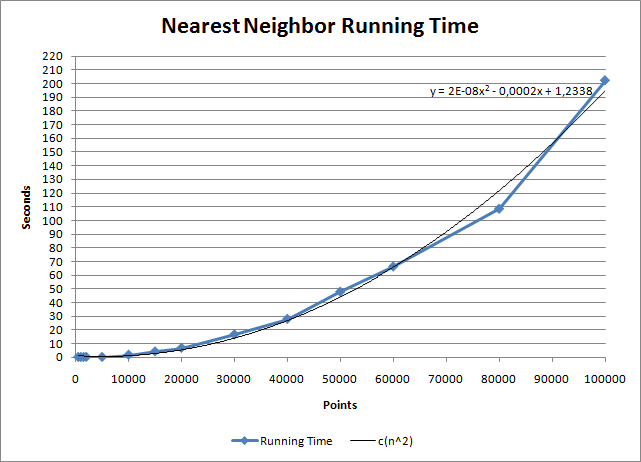
\includegraphics[scale = 0.6]{1NearestNeighbor/nnRuntimegraph.png}\\
    Figure 1: Graph of Nearest Neighbor Running Time
    \end{center}

    \noindent This graph tells us that our analysis of the running time (\ref{sub:running_time_analysis}) is correct: when the number of input points are doubled, the running time is quadrupled $(2^2)$, when they are tripled, the running time is multiplied by roughly $3^2$, etc.\\
    Along with the resulting graph of the test, we introduced a trend line (which is a $n^2$ function fitted to our test results) to show the running time is indeed $O(n^2)$.\\
    So, we can conclude that in practice this algorithm is $O(n^2)$ too.

    \subsection{Correct output}
    We analyzed a few test-cases that failed giving the correct output.\\
    We give suggestions as to what caused this behavior, and supply possible solutions below.\\

    \begin{center}
      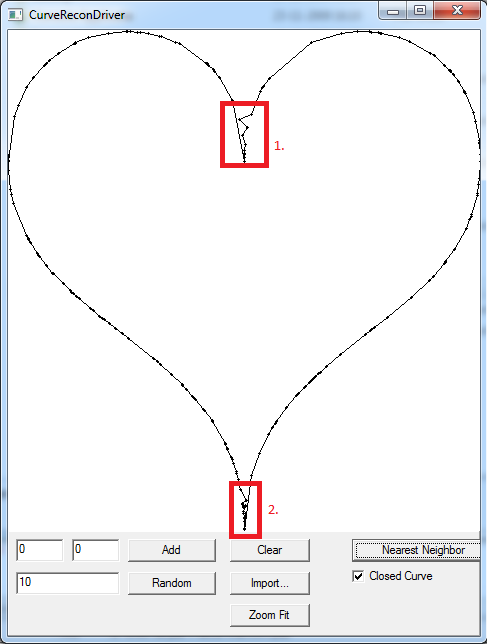
\includegraphics[scale = 0.6]{1NearestNeighbor/nnHeartgraph.png}\\
      Figure 2: Incorrect heart
    \end{center}

    \noindent An example of a test-case in which the NearestNeighbor fails is the Heart with 200 points. As you can see in Figure 2 there are 2 places the curve starts zigzagging between points.
    This problem occurs because the correct point in this case is not the nearest neighbor of the previous one. This could be corrected by taking the curve's current direction into account. This way, we could prevent the curve from jumping around.\\

    \begin{center}
      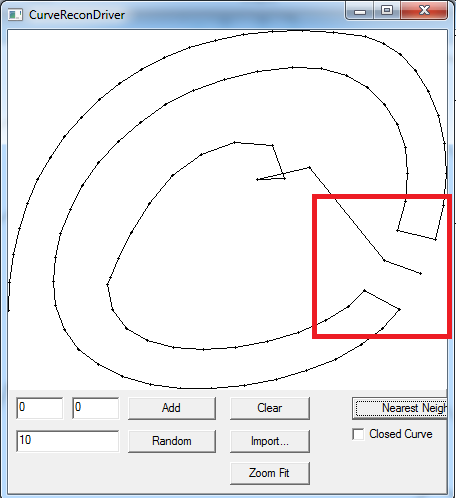
\includegraphics[scale = 0.6]{1NearestNeighbor/nnSpiralgraph.png}\\
      Figure 3: Incorrect spiral
    \end{center}

    \noindent Another failed test-case is the Spiral with 91 points. Here, we experience the same problem as in the first case, that is, going in the wrong direction because the nearest point is not the correct successor. We also see another problem caused by this: when the spiral is nearly complete, the algorithm picks the points, which haven't been processed yet. In this case those points reside at the other side of the spiral.\\

    \begin{center}
      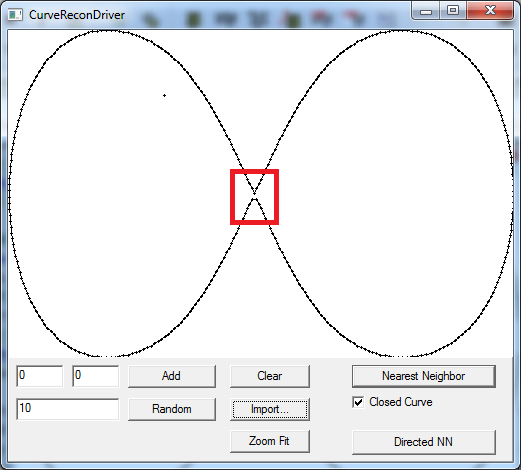
\includegraphics[scale = 0.6]{1NearestNeighbor/nnEightgraph.png}\\
      Figure 4: Incorrect eight
    \end{center}

    \noindent The third test-case is the ``8'' with 364 points. The problem here is that is does not intersect. Nearest Neighbor does not make sure there is at least one intersection. So, another thing we should take into consideration is that we need to check for intersections. \\

    \begin{center}
      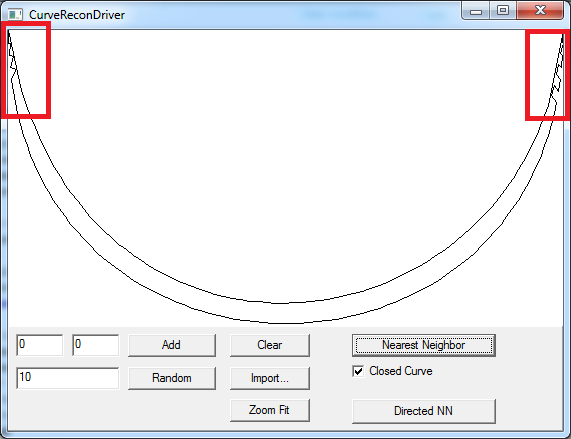
\includegraphics[scale = 0.6]{1NearestNeighbor/nnFlatgraph.png}\\
      Figure 5: Incorrect flat
    \end{center}

    \noindent The fourth and last test-case we discuss is the Flat with 178 points. This problem could also be solved by keeping track of the curve's current direction, so that it will not end up zigzagging again (marked in Figure 5).

    \subsection{Conclusion from tests}
    From all these test results we can conclude there are a number of things that need improving. We could, for example (as mentioned before), look at the curve's direction, which would fix the zigzagging. We should also check for intersections when the input requires it. 